\begin{frame}
\frametitle{Aktiver Tiefpass}
\framesubtitle{}
    \begin{block}{Aktiver Tiefpass 4. Ordnung (3dB-Tschebyscheff)}
         \begin{itemize}
             \item starker Filter mit steil Abfallenden Flanken
             \item aufgebaut aus 2 Stufen
         \end{itemize}
    \end{block}
\end{frame}
\begin{frame}
\frametitle{Versuchsaufbau}
\framesubtitle{}
    \begin{block}{Versuch}
        \begin{itemize}
            \item Analyse der einzelnen Stufen
            \item Analyse der Reihenschaltung
        \end{itemize}    
    \end{block}
    \begin{figure}[H]
    \begin{center}
            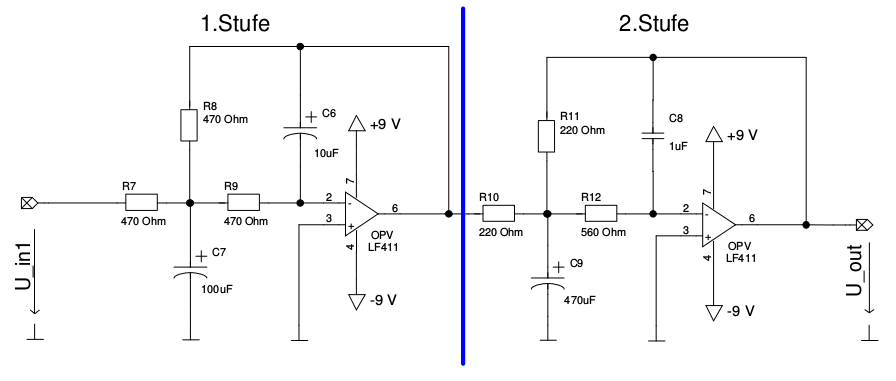
\includegraphics[scale=0.3]{./img/schaltung/tiefpass.png}
    \end{center}
    \end{figure}
\end{frame}

\begin{frame}
\frametitle{1.Stufe}
\framesubtitle{}
\begin{block}{Ergebnisse}
    \begin{itemize}
        \item Theoretische Formeln sind lang und kompliziert, daher werden hier
        nur die Ergebnisse gezeigt
    \end{itemize}
\end{block}
\end{frame}

\begin{frame}
\frametitle{1.Stufe}
\framesubtitle{}
    \begin{block}{1.Stufe}
        \begin{tabular}{c|c|c}
        & Theorie & Messung \\ 
        \hline
        Welligkeit &1.10 &1.18 \\
        Dämpfung pro Dekade &-40.50 & -40.47\\
        Grenzfrequenz &13.91 & 15.24
        \end{tabular}
    \end{block}
\begin{columns}[c]
    \column{0.5\textwidth} 
    \begin{figure}[H]
    \begin{center}
            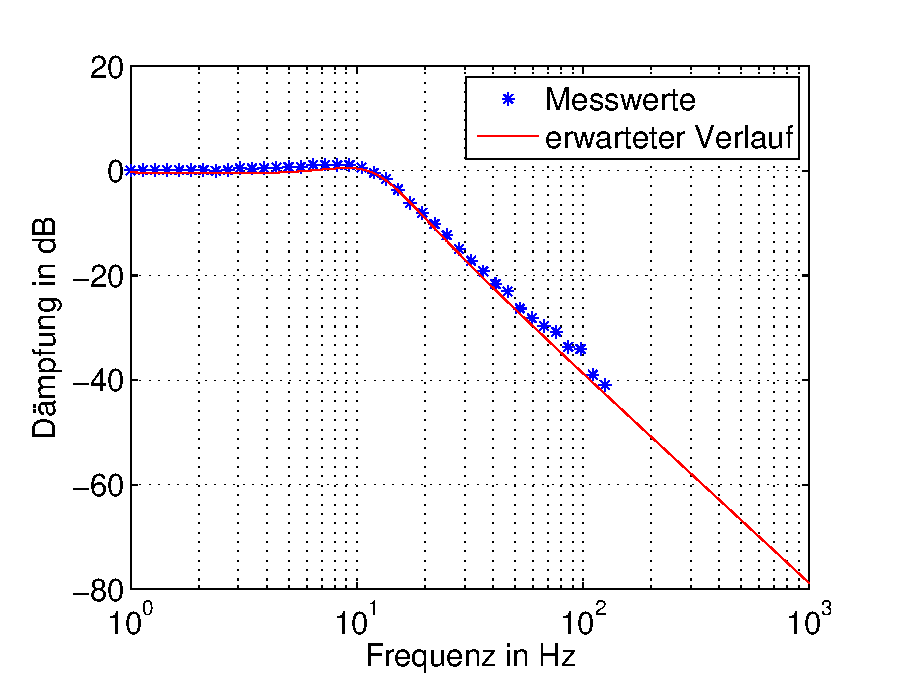
\includegraphics[scale=0.3]{./img/plots/Auf_4_bode_links_db.eps}
    \end{center}
    \end{figure}
    \column{0.5\textwidth} 
    \begin{figure}[H]
    \begin{center}
            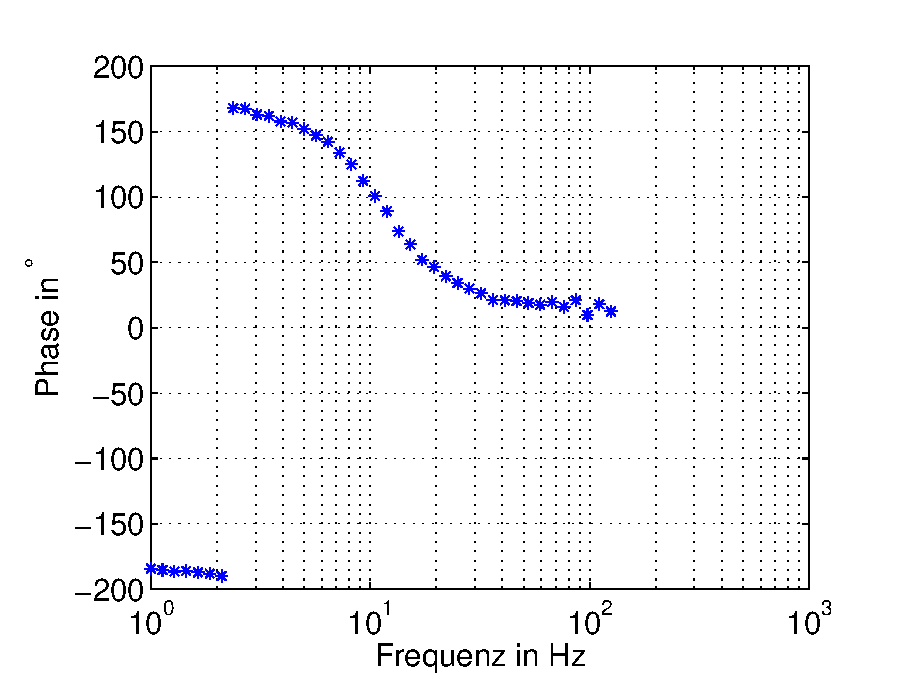
\includegraphics[scale=0.3]{./img/plots/Auf_4_bode_links_ph.eps}
    \end{center}
    \end{figure}
\end{columns}
\end{frame}

\begin{frame}
\frametitle{2.Stufe}
\framesubtitle{}
    \begin{block}{2.Stufe}
        \begin{tabular}{c|c|c}
        & Theorie & Messung \\ 
        \hline
        Welligkeit & 15.05&12.34 \\
        Dämpfung pro Dekade & -46.29& -44.98\\
        Grenzfrequenz & 32.31& 36.244
        \end{tabular}
    \end{block}
\begin{columns}[c]
    \column{0.5\textwidth} 
    \begin{figure}[H]
    \begin{center}
            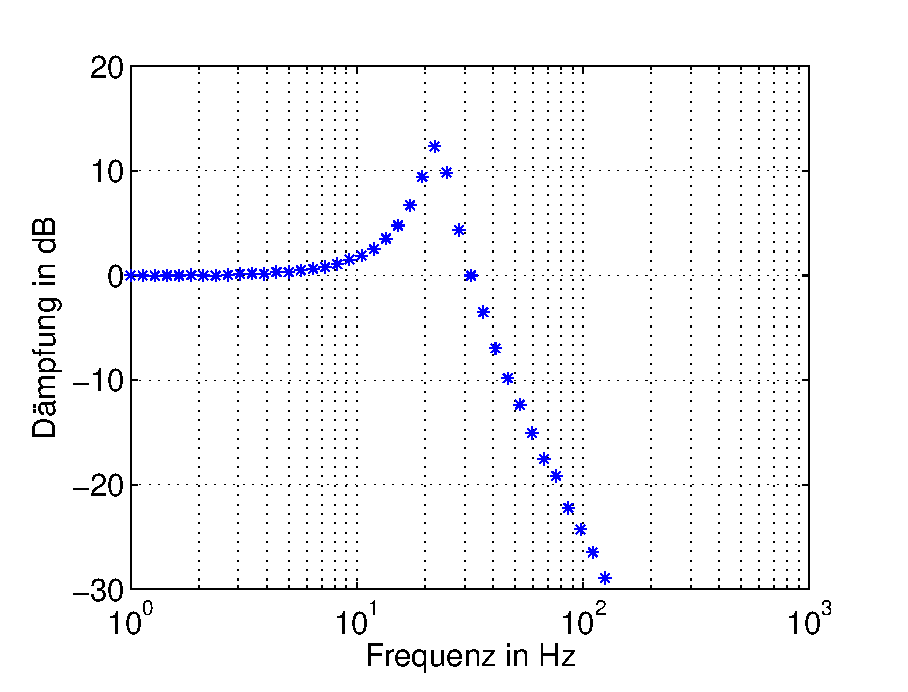
\includegraphics[scale=0.3]{./img/plots/Auf_4_bode_rechts_db.eps}
    \end{center}
    \end{figure}
    \column{0.5\textwidth} 
    \begin{figure}[H]
    \begin{center}
            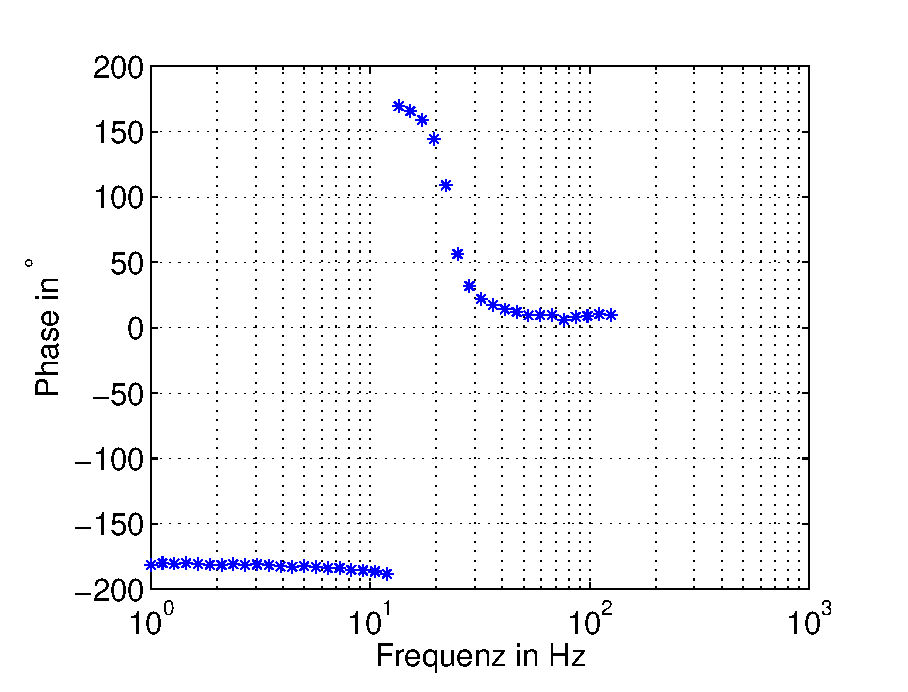
\includegraphics[scale=0.3]{./img/plots/Auf_4_bode_rechts_ph.eps}
    \end{center}
    \end{figure}
\end{columns}
\end{frame}

\begin{frame}
\frametitle{Gesamtschaltung}
\framesubtitle{}
    \begin{block}{Gesamtschaltung}
        \begin{tabular}{c|c|c}
        & Theorie & Messung \\ 
        \hline
        Welligkeit & 4.69& 2.64\\
        Dämpfung pro Dekade & -90.80& -89.63\\
        Grenzfrequenz &23.48 &25.0
        \end{tabular}
    \end{block}
\begin{columns}[c]
    \column{0.5\textwidth} 
    \begin{figure}[H]
    \begin{center}
            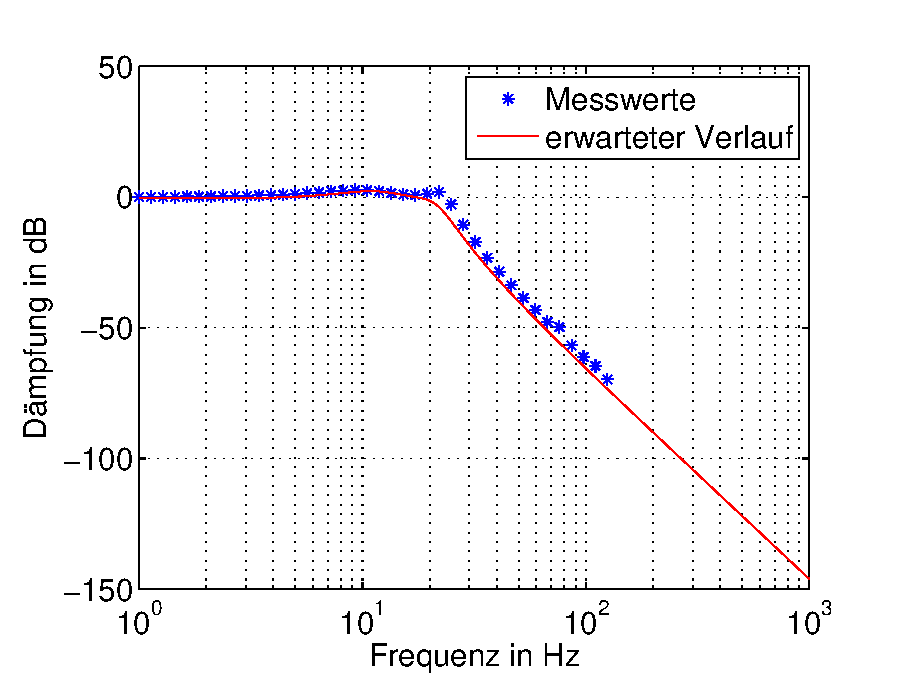
\includegraphics[scale=0.3]{./img/plots/Auf_4_bode_ges_db.eps}
    \end{center}
    \end{figure}
    \column{0.5\textwidth} 
    \begin{figure}[H]
    \begin{center}
            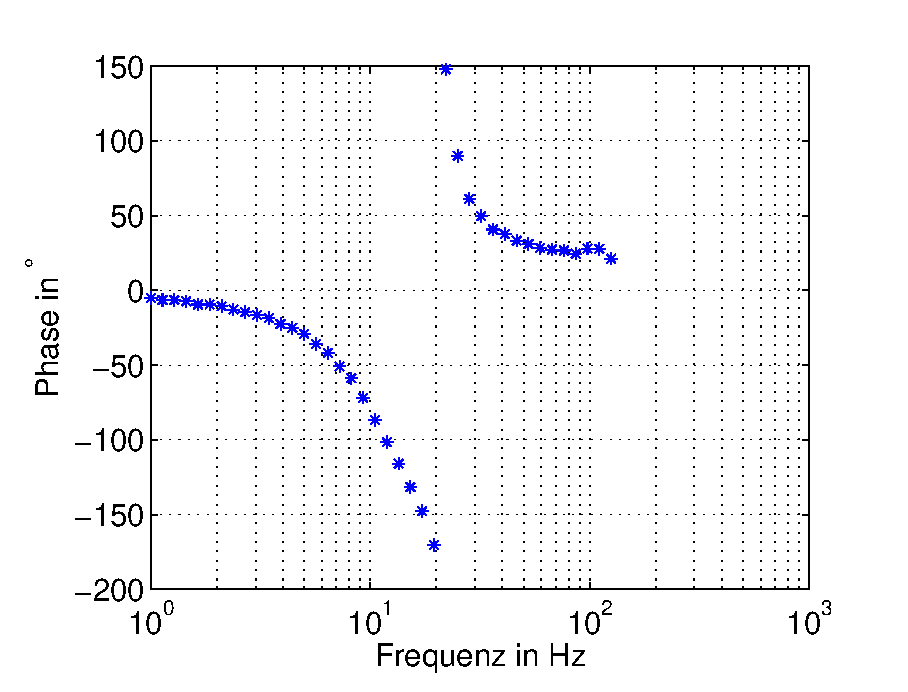
\includegraphics[scale=0.3]{./img/plots/Auf_4_bode_ges_ph.eps}
    \end{center}
    \end{figure}
\end{columns}
\end{frame}
\begin{frame}
\frametitle{Vergleich}
\framesubtitle{}
\begin{block}{}
    Vergleich $20Hz$ und $50Hz$
\end{block}
\begin{columns}[c]
    \column{0.5\textwidth}
        \begin{figure}[H]
        \begin{center}
                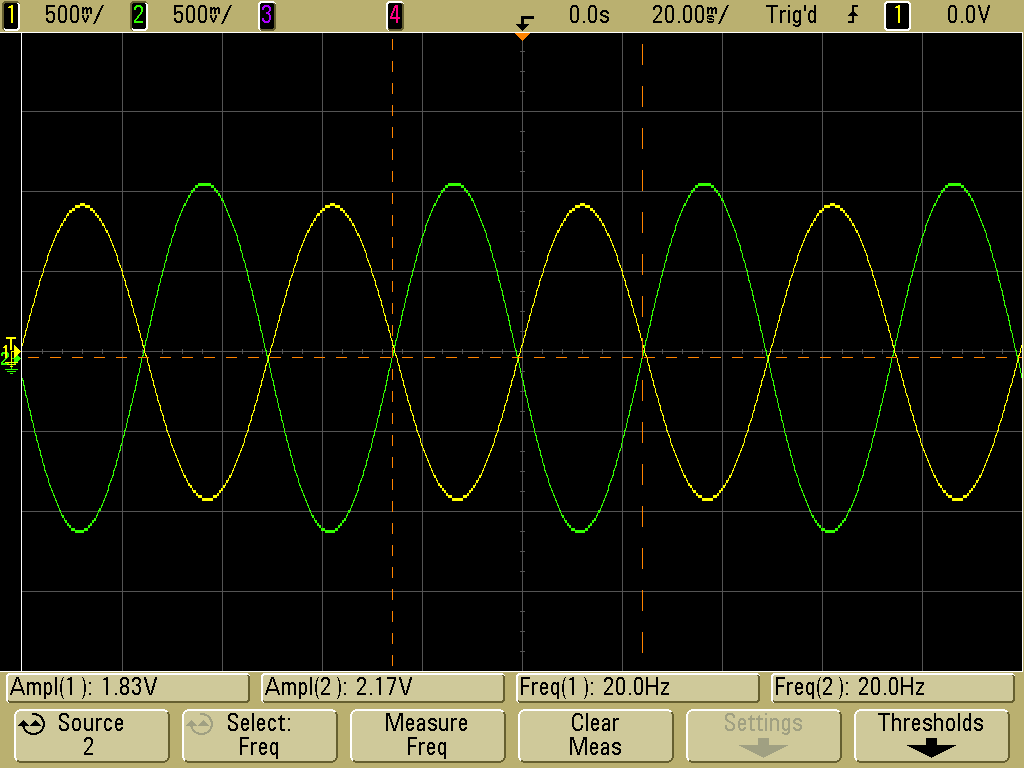
\includegraphics[scale=0.15]{./img/oszi/scope_5.png}
        \end{center}
        \end{figure}
    \column{0.5\textwidth}
        \begin{figure}[H]
        \begin{center}
                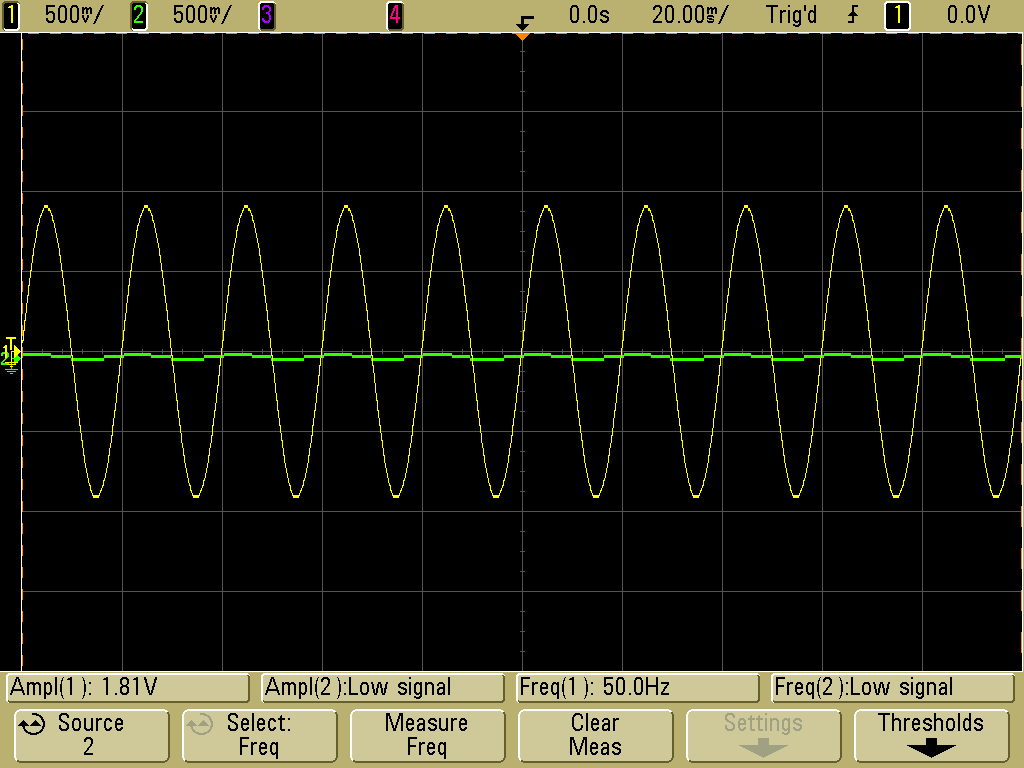
\includegraphics[scale=0.15]{./img/oszi/scope_7.png}
        \end{center}
        \end{figure}
\end{columns}

\end{frame}
